% *********************************************************************
% © 2016–2026 Jeremy Sylvestre
%
% Permission is granted to copy, distribute and/or modify this document
% under the terms of the GNU Free Documentation License, Version 1.3 or
% any later version published by the Free Software Foundation; with no
% Invariant Sections, no Front-Cover Texts, and no Back-Cover Texts. A
% copy of the license is included in the appendix entitled “GNU Free
% Documentation License” that appears in the output document of this
% PreTeXt source code. All trademarks™ are the registered® marks of
% their respective owners.
%
% *********************************************************************
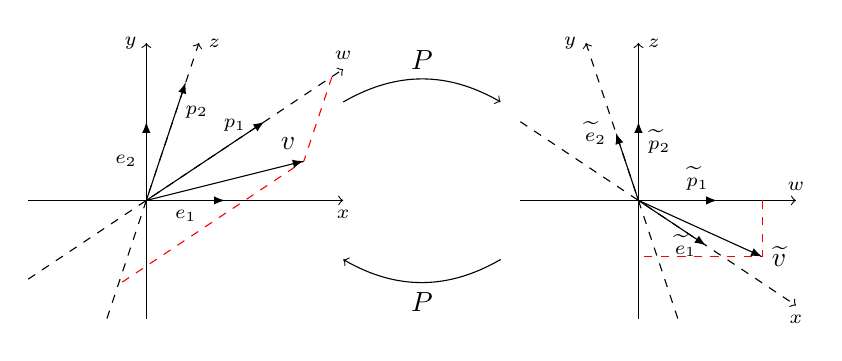
\begin{tikzpicture}[
	point/.style={circle,draw,very thin,fill,inner sep=0pt,minimum size=4pt},
	vector/.style={-latex},
]

	\draw[->] (-1.5,0) to (2.5,0) node[below] {$\scriptstyle x$};
	\draw[->] (0,-1.5) to (0,2) node[left] {$\scriptstyle y$};

	% slope: 1 over, 3 up
	\draw[dashed,->] (-0.5,-1.5) to (0.667,2) node[right] {$\scriptstyle z$};
	% slope: 3 over, 2 up
	\draw[dashed,->] (-1.5,-1) to (2.5,1.667) node[above] {$\scriptstyle w$};

	\draw[red,dashed] (2.357,1.571) to (2,0.5) to (-0.357,-1.071);
	% slope: over 2 up 1
	\draw[vector] (0,0) to node[above, near end, xshift=0.3cm, yshift=0.15cm] {$\uvec{v}$} (2,0.5);

	\draw[vector] (0,0) to node[below] {$\scriptstyle \uvec{e}_1$} (1,0);
	\draw[vector] (0,0) to node[left] {$\scriptstyle \uvec{e}_2$} (0,1);

	\draw[vector] (0,0) to node[above, near end] {$\scriptstyle \uvec{p}_1$} (1.5,1);
	\draw[vector] (0,0) to node[right, near end] {$\scriptstyle \uvec{p}_2$} (0.5,1.5);

	\begin{scope}[xshift=6.25cm]
		\draw[->] (-1.5,0) to (2,0) node[above] {$\scriptstyle w$};
		\draw[->] (0,-1.5) to (0,2) node[right] {$\scriptstyle z$};
		% slope: 3 over, 2 up
		\draw[dashed,->] (-1.5,1) to (2,-1.333) node[below] {$\scriptstyle x$};
		% slope: 1 over, 3 up
		\draw[dashed,->] (0.5,-1.5) to (-0.667,2) node[left] {$\scriptstyle y$};
		\draw[vector] (0,0) to (0.857,-0.571) node[left] {$\scriptstyle \widetilde{\uvec{e}}_1$};
		\draw[vector] (0,0) to (-0.286,0.857) node[left] {$\scriptstyle \widetilde{\uvec{e}}_2$};
		\draw[vector] (0,0) to node[above, near end] {$\scriptstyle \widetilde{\uvec{p}}_1$} (1,0);
		\draw[vector] (0,0) to node[right, near end] {$\scriptstyle \widetilde{\uvec{p}}_2$} (0,1);
		\draw[red,dashed] (1.571,0) to (1.571,-0.714) to (0,-0.714);
		\draw[vector] (0,0) to (1.571,-0.714) node[right] {$\widetilde{\uvec{v}}$};
	\end{scope}

	\draw[->] (2.5,1.25) to [out=30,in=150] node[above] {$\inv{P}$} (4.5,1.25);
	\draw[->] (4.5,-0.75) to [out=-150,in=-30] node[below] {$P$} (2.5,-0.75);

\end{tikzpicture}
